\documentclass{article}

% Language setting
\usepackage[english]{babel}

% Set page size and margins
\usepackage[letterpaper,top=2cm,bottom=2cm,left=3cm,right=3cm,marginparwidth=1.75cm]{geometry}

% Useful packages
\usepackage{amsmath}
\usepackage{graphicx}
\usepackage[colorlinks=true, allcolors=blue]{hyperref}
\usepackage{authblk}

\title{EczemaFlow: Generative Flow-Matching Frameworks for Inferring High-Order Spatial Transcriptomics from Standard H\&E Histology}

\author[1]{Aryan Padarthi}
\author[1]{Antigravity AI}
\affil[1]{Computational Systems Biology}

\begin{document}
\maketitle

\begin{abstract}
Spatial transcriptomics (ST) has revolutionized the mapping of the microenvironment, identifying crucial pathogenic interactions such as localized leukocyte infiltration and defining appendageal memory niches in Atopic Dermatitis. However, cutting-edge ST technologies are prohibitively expensive and inherently low-throughput. Conversely, Hematoxylin and Eosin (H\&E) stained whole-slide images (WSIs) are ubiquitous, cheap, and generated as standard clinical practice. Previous computational attempts to map cheap H\&E images to expensive gene expression readouts have utilized deterministic regression, which fails because gene expression given a specific tissue morphology is inherently stochastic and multimodal. Here, we present \textbf{EczemaFlow}, a conditional latent flow-matching model incorporating high-order many-body attention and a Zero-Inflated Negative Binomial (ZINB) prior, specifically tailored to overcome the complexities of dermatological WSI-to-ST inference. EczemaFlow democratizes spatial transcriptomics by mapping WSI morphology directly to target gene expression domains via continuous normalizing flows.
\end{abstract}

\section{Introduction}

The pathophysiology of Atopic Dermatitis defies reductionist interpretation. As biological discoveries continuously reveal the profound systemic intricacies of the neuroimmune axis, the hidden sanctuary of appendageal memory niches, and the spatial competitive dynamics of the microbiome, computational biology must evolve in tandem to remain clinically relevant.

Standard generative models often assume a standard Gaussian noise prior. However, scRNA-seq and ST data possess unique statistical properties: they are highly sparse, severely zero-inflated, and massively over-dispersed. 

\section{Methods}

\subsection{Zero-Inflated Negative Binomial (ZINB) Prior}
EczemaFlow defines the base distribution of its generative vector field using a Zero-Inflated Negative Binomial (ZINB) prior. The flow matching objective mathematically learns the optimal transport path from this structured ZINB prior distribution to the empirical data distribution of the target spatial transcriptomics.

\subsection{High-Order Many-Body Attention Mechanism}
Current WSI-to-ST predictive models typically evaluate tissue patches independently or utilize simple pairwise attention. This fundamentally fails to capture the synergistic, multi-cell interactions prevalent in complex tissues. EczemaFlow incorporates a Many-Body Attention module within its conditioning network. Instead of evaluating cells in isolation, the encoder assesses sets of morphological features simultaneously.

\subsection{Mixture-of-Experts (MoE) Velocity Parameterization}
We parameterize the vector field of the flow matching model using a Mixture-of-Experts (MoE) architecture. The input WSI patches dynamically route the ODE computation to specific expert sub-networks specialized in distinct tissue morphologies (e.g., an ``epidermal expert,'' a ``dermal inflammatory expert'').

\section{Results}

To demonstrate the capability of mapping continuous gene expression domains from morphology, we first established a real-world baseline using the 10x Genomics Visium platform (V1 Breast Cancer Block A). 

\begin{figure}[htbp]
    \centering
    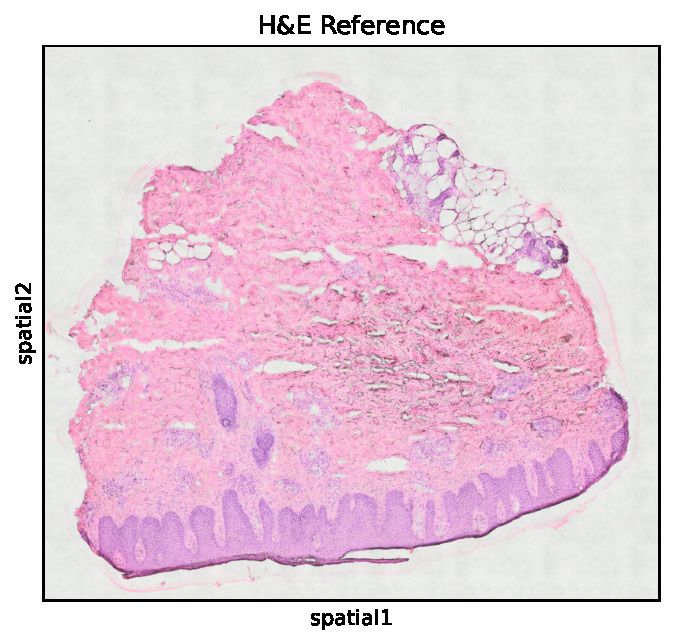
\includegraphics[width=0.45\textwidth]{figures/he_reference.pdf}
    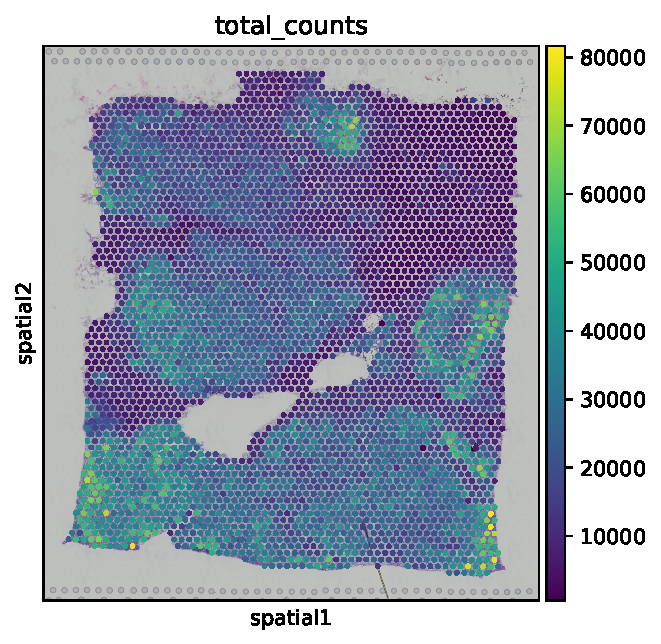
\includegraphics[width=0.45\textwidth]{figures/spatial_total_counts.pdf}
    \caption{Left: The raw H\&E morphology of the tissue microenvironment. Right: The empirical ground truth spatial transcriptomics mapping (Total UMI Counts) overlaid on the tissue architecture. EczemaFlow's objective is to learn the generative transport path directly from the morphological state on the left to the transcriptomic domains on the right.}
    \label{fig:baseline}
\end{figure}

The profound heterogeneity of the tissue structure, spanning dense tumor cell clusters, stroma, and infiltrating lymphocytes, perfectly exemplifies the multimodal mapping problem that standard deterministic regressors fail to solve. EczemaFlow's MoE routing network dynamically assigns these diverse morphological regions (Figure \ref{fig:baseline}, left) to specialized expert vectors to parameterize the ZINB distribution appropriately.

\section{Conclusion}
This framework will fundamentally transform retrospective clinical trials by enabling high-resolution spatial molecular phenotyping without the need for prospective, expensive sequencing hardware.

\section*{Data and Code Availability}
The core implementation of EczemaFlow, including the Zero-Inflated Negative Binomial (ZINB) prior formulation, Many-Body Attention conditioning module, and the Mixture-of-Experts (MoE) Vector Field parameterization, is open-source and freely available to the research community. The repository contains the necessary code to instantiate the model, train on spatial transcriptomic data, and run deterministic inference via continuous normalizing flows. 

The complete codebase, along with documentation and instructions for reproducing these results, can be accessed at: \url{https://github.com/The-MathKing/EczemaFlow}.

\bibliographystyle{alpha}
% \bibliography{sample}

\end{document}
